\chapter{Background}
\label{background}

\begin{quote}
This chapter introduces the general context of text classification problem. I present the motivation for the fashion news popularity prediction. In addition, a brief introduction of the concept drift is given. Also, a detailed review of some latest concept drift detectors is presented. In addition, basic theory of deep learning model and its application in natural language is discussed. An introduction of some latest deep learning models in text classification is presented at last.
\end{quote}

\section{Concept Drift}
\subsection{Definition}
\subsection{Algorithms}
As of today, many concept drift have been proposed. Most of the concept drift detectors are composed of two parts. One is a base learner, such as decision tree~\cite{wang2003mining}, support vector machine~\cite{klinkenberg2000detecting}, which is used to classify the incoming data. Then, The prediction result is compared with the true label and compute the metrics. Another part is the drift detection method which indicate whether the concept drift occurs or not based on the classification result. If the concept drift occurs, according to different detector framework, the base learner will re-trained in a new subset of the instances. For each incoming instance, the framework repeat the process. 

According to the number of citations, there are eight popular concept drift detectors, DDM~\cite{gama2004learning}, EDDM~\cite{baena2006ear}, PHT~\cite{page1954continuous}, ADWIN~\cite{bifet2007learning}, Paired Learners~\cite{bach2008paired}, ECDD~\cite{ross2012exponentially}, DoF~\cite{sobhani2011new}, and STEPD~\cite{nishida2007detecting}. The most popular and effective method is the Drift Detection Method (DDM). Its mechanism is simple and easy to understand. DDM uses a base learning (decision tree) to classify the incoming instance and the the online error-rate is computed with the prediction result. In the probably approximately correct learning model~\cite{michalski2013machine}, it is assumed that the error rate of the base learner will decrease when the number of training instance increases if the distribution of the incoming instances is stationary. Thus, if the model detects a significant increase of the online error-rate, it suggests the concept drift occurs. 

Suppose every instance in the form of $(\mathbf{x}_i, y_i)$. The base learner gives the prediction $\hat{y}_i$ that can be used to compute the error-rate $p_i$ and the standard deviation $s_i$ given by 
\begin{equation}
s_i = \sqrt{\frac{p_i(1-p_i)}{i}}
\end{equation}
If it is a binary classification problem, for the set of incoming instance, the error is a random variable from Bernoulli trails and the binomial distribution gives the probability for the random variable representing the number of errors in a sample of $n$ instances. If the number of instance is large, the Binomial distribution is closely approximated by a Normal distribution with same mean and variance. We assume the confidence level is $alpha$. Then, the confidence interval for error $p$ is about $p_i\pm\alpha*s_i$. The framework records the minimum of $p_i$ and $s_i$, obtaining $p_min$ and $s_min$, during the training process. The warning level is defined as $p_{min} + 2 * s_{min}$ by setting $\alpha$ to $95\%$. The drift level is $p_{min} + 3 * s_{min}$ with $99\%$ confidence level. Suppose a data stream where the error reaching the warning level at example $w$ and the drift level at example $d$. The base learner is re-trained using only the instances from $w$ till $d$. Based on previous experiments, DDM is proved to be the best method in datasets suffering from gradual concept drifts~\cite{Goncalves2014}.

The Early Drift Detection Method (EDDM)~\cite{baena2006ear} is similar to the Drift Detection Method (DDM). It uses the distance-error-rate rather than the online error-rate to identify the occurrence of the concept drift. While there is no concept drift, the predictions and the distance between two errors will be increased during the training process. For every incoming instance, $p'_i$, the avergae distance between two errors, and its standard deviation $s'_i$ are computed. The maximums of $p'_i$ and $s'_i$ are recorded, obtaing $p'_{max}$ and $s'_{max}$. Similar to DDM, there are also two thresholds. The threshold is defined as 
\begin{equation}
\frac{p'_i + 2 * s'_i} {p'_{max} + 2*s'_{max}}<\alpha
\end{equation}
where $\alpha$ is the confidence level. Beyond the confidence level of the warning level, the instances are stored in advance for the re-training process. Beyond the confidence level of the drift level, the base learning is re-trained using the stored examples. The EDDM is designed for dealing with the gradual concept drift. It has better performance than DDM with noise free data but worse with real world data~\cite{Goncalves2014}.


The Adaptive Windowing Method (ADWIN) is another approach for dealing with concept drift. It uses a sliding window whose size changes during the training process. The window size is recomputed online according to the rate of change observed from the data stream. The window size grows when there is no apparent concept change and decreases when the change is detected.

We assume ADWIN keeps a sliding window $W$ with size of $n$. $\hat{\mu}_W$ is the average of the instance in $W$ while $\mu_W$ is the average of $\mu_t$ for $t \in W$. When two large enough sub-windows $W_0$ and $W_1$ exhibit distinct enough averages, the old portion window is drop. The value of $\epsilon_{cut}$ for a partition $W_0 \cdot W_1$ of $W$ is computed as follows

\begin{equation}
\epsilon_{cut} = \sqrt{\frac{1}{2m} \cdot \mbox{ln} \frac{4}{\epsilon'}}
\end{equation} 
where $\epsilon$ is the confidence level, $m = \frac{1}{1/n_0 + 1/n_1}$, $n_0$ and $n_1$ are the length of the corresponding sub-windows. For each time-step, the new incoming instance is added to the head of $W$ and the elements from the tail is dropped one by one until $|\hat{\mu}_{W_0} - \hat{\mu}_{W_1}| \geq \epsilon_cut$ holds. ADWIN is memory-efficient and it is the fastest one of these four popular algorithm. In some real world problem, it is even faster than the base learner~\cite{Goncalves2014}. 

The Paired Learner is a slightly different framework which uses two learners, a stable learning predicting based on all instances and a reactive learned predicts based on some recent instances with a fixed window size. The PL method has a circular list of bits with the same length of the window which stores $1$ if the example is misclassified by the stable learner but classified by the reactive learner correctly, and $0$ otherwise.
While the number of $1$ is great than the threshold $\theta$, it indicates the concept drift occurs. Then, the stable learner is substituted by the reactive one and the circular list is set to $0$. 

Though the paired learner is a very creative method compared with other approaches. It is the worst methods dealing with the abrupt concept drift. As it uses two learner, PL is the slowest among these methods.

\section{Deep Learning Models in Text Classification}

Deep learning refers to the machine learning techniques for learning and utilizing neural networks with multiple layers, such as deep neural network (DNN), convolutional neural network (CNN), recurrent neural network (RNN). Deep learning has proven effective in reshaping the processing of speech recognition, and machine vision in a revolutionary way. In speech, image, deep learning effectively addresses the semantic gap problem by learning high-level concepts from raw data in a direct manner. Compared with these tasks, natural language processing is less straightforward as it is doubtful whether the neural representations learned from textual data can provide equally direct insight onto natural language. 

However, recently, deep learning has been successfully applied to the NLP problem and some significant achievements have been made. There are five main tasks in NLP, including translation, matching, classification, structured prediction and the sequential decision process~\cite{Li2017}. The deep learning technique has proven to outperformed in the first four tasks. Because in traditional machine learning, features are designed by humans and feature engineering is bottleneck, require much human experience. Deep learning break away these difficulties by using deep model structure. End-to-end training and representation learning really e it powerful machinery for NLP.

Text classification is an import task in NLP. It has a variety of applications, including web search, ranking, recommendation system, document classification. Recently, many deep learning models in text classification problem has been proposed~\cite{Joulin2016}\cite{zhang2015character}. each of them achieves good performance and has its own pros and cons. In this section, four latest text classification models using deep learning techniques are introduced. Meanwhile, the fundamental deep learning technologies are discussed. 


\subsection{fastText}

fastText, as its name would suggest, is a fast text classification model developed by Facebook AI Research. While other deep learning models tend to be slow to train and test which significantly limits their usage on large scale datasets. fastText can be trained on more than one billion words in less than ten minutes using a standard multicore CPU, and classify half a million sentences among 312k classes in less than a minutes.

The structure of fastText is shown in Figure \ref{fasttext_structure}. Different with other deep learning models which just use all words as the input features, fastText uses a bag of n-grams as additional features to capture the partial information about the word order. For example, for a sentence like ``I like eating apples'', the bag of 2-grams includes ``I like'', ``like eating'', ``eating apples''. Therefore, the input features are [``I'', ``like'', ``eating'', ``apples'', ``I like'', ``like eating'', ``eating apples'']. With this trick, the classifier can easily distinguish the difference between ``Jerry loves Tom'' and ``Tom loves Jerry''.

\begin{figure}
\centering
\caption{Model structure of fastText for a sentence with $N$ n-gram features.}
\label{fasttext_structure}
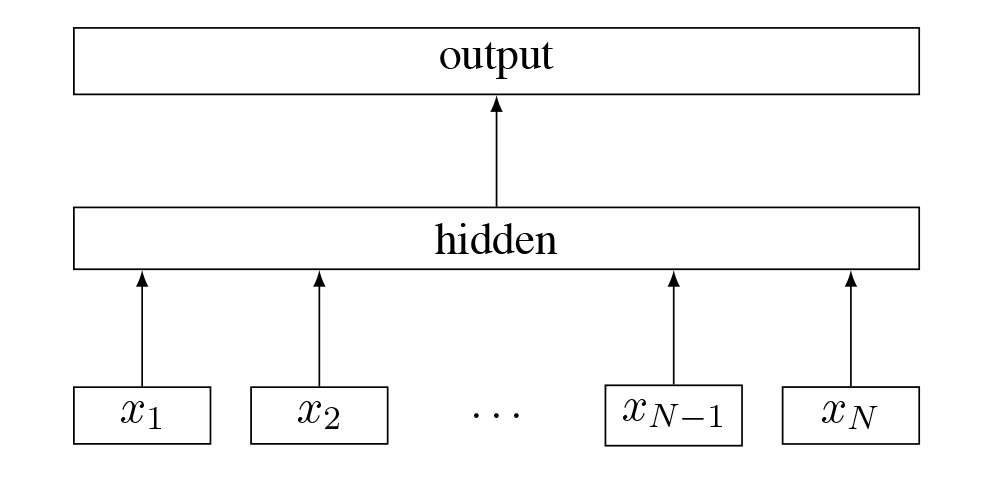
\includegraphics{fasttext_structure.png}

\end{figure}

Then every word and n-gram is transformed into a corresponding number and feed into the embedding layer. Simply speaking, embedding is just sparse matrix multiplication. For each word or n-gram, it corresponds to an unique number. The number can be represented as a one-hot coding vector. We assume the word of ``apples'' corresponds to number of $2$ and there are totally 6 words and n-grams in our corpus. The one-hot vector $\mathbf{v}$ for ``apples'' is $[0, 1, 0, 0, 0, 0]$. There is only one element can be $1$ and others are $0$. Each position is a word and the length of $v$ is the corpus size. As the number of ``apples'' is $2$, the second element of the vector is $1$. To embed a word or n-gram, we simply do
\begin{equation}
\label{embed}
\mathbf{f} = \mathbf{W} \mathbf{v}
\end{equation}
where $\mathbf{f}$ is the embedded word vector, $\mathbf{W}$ is a $D \times \mbox{corpus size}$ matrix and $D$ is the dimension of the embedded vector for each word. After the embedding layer, each word obtains a unique embedded word vector and fastText averages these vectors. The averaged vector is called text representation which stores the features of the whole sentences. Finally, the text representation is in turn fed to a linear classifier. The softmax function is used to compute the probabilities of each class. For text representation in form of $\mathbf{e}$, the probability of class $j$ is shows as follows
\begin{equation}
p(y=j|\mathbf{f}) = \frac{e^{\mathbf{f}^\intercal \mathbf{w}_j}} {\sum_{k=1}^K e^{\mathbf{f}^\intercal\mathbf{w}_k}}
\end{equation}
where $\mathbf{w}$ is a weighting vector, $K$ is the number of classes. 

fastText uses the negative log-likelihood as the loss function. For a set of $N$ instances, the loss function is defined as 
\begin{equation}
-\frac{1}{N}\sum_{n=1}^{N}y_n\mbox{log}({p_{y_n}})
\end{equation}
where $y_n$ is the ground truth of the example $n$. The model is trained by using stochastic gradient descent. To increasing the convergence speed, the linear learning rate decay is applied.

For a large number of classes, fastText uses hierarchical softmax to improve the efficiency in computing the linear classifier. As, in our experiment, the number of classes is so small that hierarchical softmax has no obvious advantages, we will not discuss it in this chapter.

\subsection{Character-level Convolutional Network}
Different with most of the deep learning models which deal with the inputs on word level, Character-level Convolutional Network (Char-CNN) treats text as a kind of raw signal at character level and applies deep convolutional networks (ConvNets) on them. Compared with conventional machine learning methods and other deep learning models, Char-CNN has many advantages. Firstly, as the inputs are treated as signal on character-level, 
Char-CNN does not require the knowledges of words. Secondly, previous research proves that the knowledge about syntactic or semantic structure of a language are not required in ConvNets. Thirdly, as the model accepts a sequence of characters which are encoded by prescribing an alphabet for the text, Char-CNN can deal with different language. Fourthly, the model only works on character level, thus, it can easily learn the abnormal character combinations such as emoticons and misspellings.

\begin{figure}
\centering
\caption{The model architecture of Character-level Convolutional Network~\cite{zhang2015character}}
\label{char_cnn}
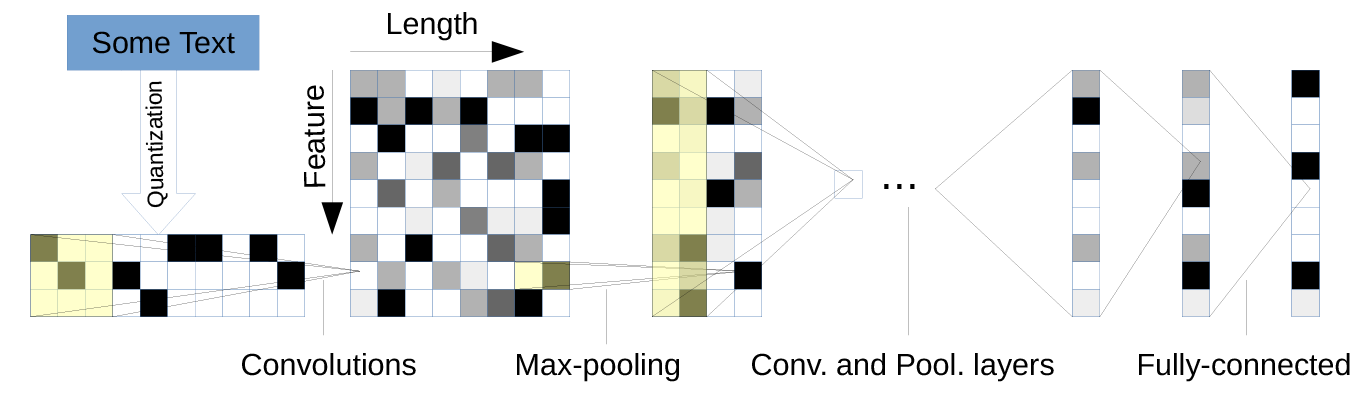
\includegraphics{char_cnn.png}
\end{figure}

The architecture of the Char-CNN is shown in Figure \ref{char_cnn}. The model receives the text and quantize each character. This pre-process is called character quantization which is done by prescribing an alphabet of size $m$ for the raw text, and each character is quantized into one-hot encoding. For English text, we normally use the alphabet consisting 70 characters, which is presented as follows
\begin{lstlisting}[language=Python]
  abcdefghijklmnopqrstuvwxyz0123456789
  -,;.!?:"/\|_@#$&*~`+-=<>()[]{}'^%
\end{lstlisting}
There are 26 English letters, 10 digits, 33 other characters and the new line character, which is not shown above. For example, the character ``b'' is quantized into [0,1,0,0,0,.....,0]. Only the second element has value of 1 while other elements are all zero. 

The encoded text is fed to the convolutional and the maxpooling layers after the quantization. These two layers are the key components of the ConvNets. In Char-CNN, the temporal, as known as one-dimensional, convolutional modules are used. The temporal convolution is similar to the convolutions commonly used in computer vision, which just simply computes a 1-D convolution. For a input function and a kernel function in form of $g(x)\in[1,l] \rightarrow \mathbb{R}$ and $f(x) \in [1,k] \rightarrow \mathbb{R}$, where $l$ is the input feature size and $k$ is the kernel size. The convolution function $h(y) \in [1, \frac{l-k}{d}+1] \rightarrow \mathbb{R}$ is defined as 
\begin{equation}
h(y) = \sum_{x=1}^{k} f(x) \cdot g(y \cdot d -x + c)
\end{equation}
where $d$ is the stride, $c$ is an offset constant which is defined as
\begin{equation}
c = k-d+1
\end{equation}
For a ConvNets with input feature size of $m$ and output feature size of $n$, each inputs and outputs element are $g_i(x)$ and $h_j(y)$ correspondingly. And the weight of the kernel is $f_{i,j}(x)$ where $i=1,2,...,m$ and $j=1,2,...,n$. The output $h_j(y)$ is the sum over $i$ of the convolutions between $g_i(x)$ and $f_{i,j}(x)$.	As objects tend to have a local spatial support, for example, the connect between each characters in a word, such computation can extract the local features which makes ConvNets so powerful.

After the convolutional layer, it is the temporal max-pooling layer which helps us to train deeper models. Pooling is a effective method used to combine several nearby features into a local global `bag of features' to preserve task-related information while removing irrelevant information. For example, the vector $\mathbf{v}$ with $P$ components is reduced by the pooling layer $h$ to a single scalar $h(v)$. There are two main pooling way: average pooling $h(\mathbf{v}) = \frac{1}{P} \sum_{i=1}^P v_i$ and max pooling $f(\mathbf{v}) = \mbox{max}_i v_i$. The temporal max-pooling is the same as spatial max-pooling except it is in 1-D~\cite{boureau2010theoretical}. For a input function $g(x)\in[1,l] \rightarrow \mathbb{R}$, the max-pooling function $h(y) \in [1, \frac{l-k}{d}+1] \rightarrow \mathbb{R}$ is defined as 
\begin{equation}
h(y) = \mbox{max}^{k}_{x=1} g(y\cdot d -x +c)
\end{equation}

In Char-CNN, there are 6 convoltional layers and the first two convolutional layers and the last convolutional layer followed by a max-pooling layer. The configurations of the convolutional layers are presented in Table \ref{config_char_cnn}

\begin{table}[]
\caption{The configurations of the convolutional layers in Character-level Convolutional Network}
\centering
\label{config_char_cnn}
\begin{tabular}{ccccc}
Layer & Feature & Kernel Size & Pooling Size &  \\ \cline{1-4}
1     & 1024    & 7           & 3            &  \\
2     & 1024    & 7           & 3            &  \\
3     & 1024    & 3           & N/A          &  \\
4     & 1024    & 3           & N/A          &  \\
5     & 1024    & 3           & N/A          &  \\
6     & 1024    & 3           & 3            & 
\end{tabular}
\end{table}

Following the 6 convolutional layers, there are 3 fully connected layers. The non-linearity used in Char-CNN is the ReLUs which defined as 
\begin{equation}
\mbox{ReLU}(x) = \mbox{max}(0,x)
\end{equation}
The configurations of the fully connected layers is shown in Table \ref{config_char_fl}
\begin{table}[]
\caption{The configurations of the fully-connected layers in Character-level Convolutional Network}
\centering
\label{config_char_fl}
\begin{tabular}{cc}
Layer & Output units      \\ \hline
7     & 1024              \\
8     & 1024              \\
9     & Number of classes
\end{tabular}
\end{table}

All the weights in the Char-CNN is initialed by a Gaussian distribution with mean of $0$ and standard deviation of $0.05$. Same as fastText, the Char-CNN is trained by stochastic gradient descent with batch size of 128. It also uses momentum to accelerate the descent. The 0.9 momentum is initialed with the step size of 0.01, which is halved 3 epochs for 10 times.

Compared with traditional machine learning method in text classification, such as bag-of-words~\cite{sparck1972statistical}, bag-of-ngrams, bag-of-means on word embedding~\cite{mikolov2013distributed}, and some deep learning methods, such as word-level ConvNets, Long-short term memory, Character-level Convolutional Network is an effective method and it performs better than most of the traditional machine learning methods in large datasets~\cite{zhang2015character}.

\subsection{Bidirectional Long-short Term Memory Network}
\begin{figure}
\centering
\caption{The mechanism of the recurrent neural network~\cite{Greff2017}}
\label{rnn}
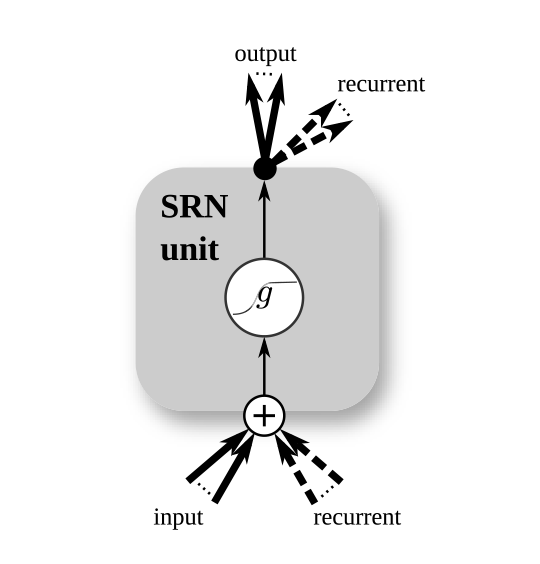
\includegraphics{rnn.png}
\end{figure}
Recurrent Neural Network (RNN) is treated as a good type of neural network to deal with sequence-like data, because it can use its internal state to process sequences of inputs and present the dynamic temporal behavior for the sequence. The basic mechanism of RNN is shown in Figure \ref{rnn}. The simplest form of RNN is an multiple layer perceptron with the previous set of the hidden unit activations feeding back into the network along with the inputs~\cite{bullinaria2013recurrent}. 

However, RNN has the gradient vanishing problem which makes it hard to train. To overcome this problem, many new types of recurrent neural networks were introduced. The Long-Short Term (LSTM) unit is one of the most effective units which was firstly proposed by Hochreiter and Schmidhuber~\cite{hochreiter1997long}. The basic idea behind LSTM units is that it introduces some gates to control the degree which the units keep the previous states and memorize the current inputs. The detailed schematic of LSTM unit is shown in Figure \ref{lstm}.
\begin{figure}
\centering
\caption{The schematic of the LSTM unit~\cite{Greff2017}}
\label{lstm}
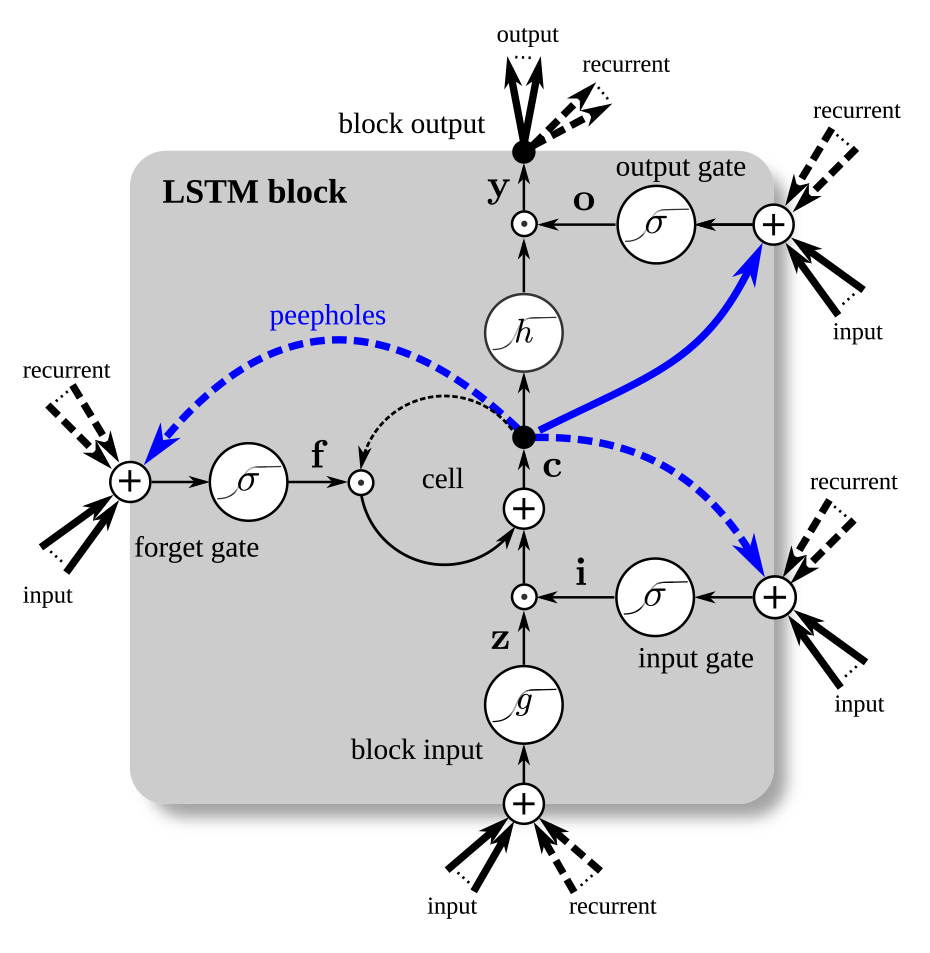
\includegraphics{lstm.png}
\end{figure}

We suppose the input vector at time $t$ is $\mathbf{x}^t$, the state at time $t-1$ is $\mathbf{h}^{t-1}$ $N$ is the number of LSTM units, and $M$ is the number of instances. There are following weights for the LSTM unit:
\begin{itemize}
	\item Input weights: $\mathbf{W}_z, \mathbf{W}_i, \mathbf{W}_f, \mathbf{W}_o \in \mathbb{R} ^{N\times M} $
	\item Recurrent weights: $\mathbf{R}_z, \mathbf{R}_i, \mathbf{R}_f, \mathbf{R}_o \in \mathbb{R}^{N\times N}$
	\item Peephole weights: $\mathbf{p}_i, \mathbf{p}_f, \mathbf{p}_o \in \mathbb{R}^{N}$
	\item Bias weights: $\mathbf{b}_z,\mathbf{b}_i, \mathbf{b}_f, \mathbf{b}_o \in \mathbf{R}^{N} $
\end{itemize}

Then the computation of LSTM layer forward propagation can be presented as
\begin{equation}
\mathbf{z}^t = g( \mathbf{W}_z \mathbf{x}^t + \mathbf{R}_z \mathbf{h}^{t-1} + \mathbf{b}_z)
\end{equation}
\begin{equation}
\mathbf{i}^t = \sigma( \mathbf{W}_i \mathbf{x}^t + \mathbf{R}_i \mathbf{h}^{t-1} + \mathbf{p_i} \odot \mathbf{c}^{t-1} + \mathbf{b}_i)
\end{equation}
\begin{equation}
\mathbf{f}^t = \sigma( \mathbf{W}_f \mathbf{x}^t + \mathbf{R}_f \mathbf{h}^{t-1} + \mathbf{p_f} \odot \mathbf{c}^{t-1} + \mathbf{b}_f)
\end{equation}
\begin{equation}
\mathbf{c}^t = \mathbf{z}^t \odot \mathbf{i}^t + \mathbf{c}^{t-1} \odot \mathbf{f}^t
\end{equation}
\begin{equation}
\mathbf{o}^t = \sigma( \mathbf{W}_o \mathbf{x}^t + \mathbf{R}_o \mathbf{h}^{t-1} + \mathbf{p_o} \odot \mathbf{c}^{t} + \mathbf{b}_o)
\end{equation}
\begin{equation}
\mathbf{h}^t = h(\mathbf{c}^t) \odot \mathbf{o}^t
\end{equation}
where $\sigma$, $g$, and $h$ are activation functions
\begin{equation}
\mbox{Logistic sigmoid: } \sigma (x) = \frac{1}{1+e^{-x}}
\end{equation}
\begin{equation}
\mbox{Hyperbolic tangent: } g (x) = h(x) = \mbox{tanh}(x)
\end{equation}
Based on this mechanism, LSTMs do not suffer from the optimization problem and can capture long-term temporal dependences. LSTMs have been applied to many difficult problem, such as handwriting generation~\cite{Graves2013}, translation~\cite{Luong2014}, speech synthesis~\cite{fan2014tts}. 

However, the disadvantage of LSTMs is that they ignore the future context as it only read the data in temporal order. To overcome this limit, Bidirectional LSTMs (BLSTM) introduces a second layer where the LSTM units process the sequence in opposite order. Based on this design, the model has the ability to extract the features both from past and future. There are two main method to combine the outputs from forward and backward propagation. One is concatenating two output into a  new vector at each time-step. Another way is using element-wise sum operator. In this case, the output at time $i$ is defined as 
\begin{equation}
\label{element_wise_sum}
\mathbf{h}^{t} = \mathbf{h}^{t,\leftarrow} \oplus \mathbf{h}^{t, \rightarrow}
\end{equation}

Zhang et al. firstly proposed a text classification model based on BLSTM~\cite{zhang2015relation}. The architecture of the model is shown in Figure \ref{blstm}. Similar to fastText model, the first layer is the embedding layer on word level. To use the knowledge of general domains, the weights of the embedding layer are initialized by the pre-trained word vector. The pre-trained word vector is obtained by the word2vector tool~\cite{Mikolov2013}. In the BLSTM layer, the output is obtained by sum the backward and forward outputs as introduced in Equation \ref{element_wise_sum}. Based on the hypothesis that only several key words and the associated features contribute to the classification, the model uses the max-pooling rather than average-pooling after the BLSTM layer to extract the semantic meaning of a sentence.
\begin{figure}
\caption{Model structure of bidirectional LSTM}
\label{blstm}
\centering
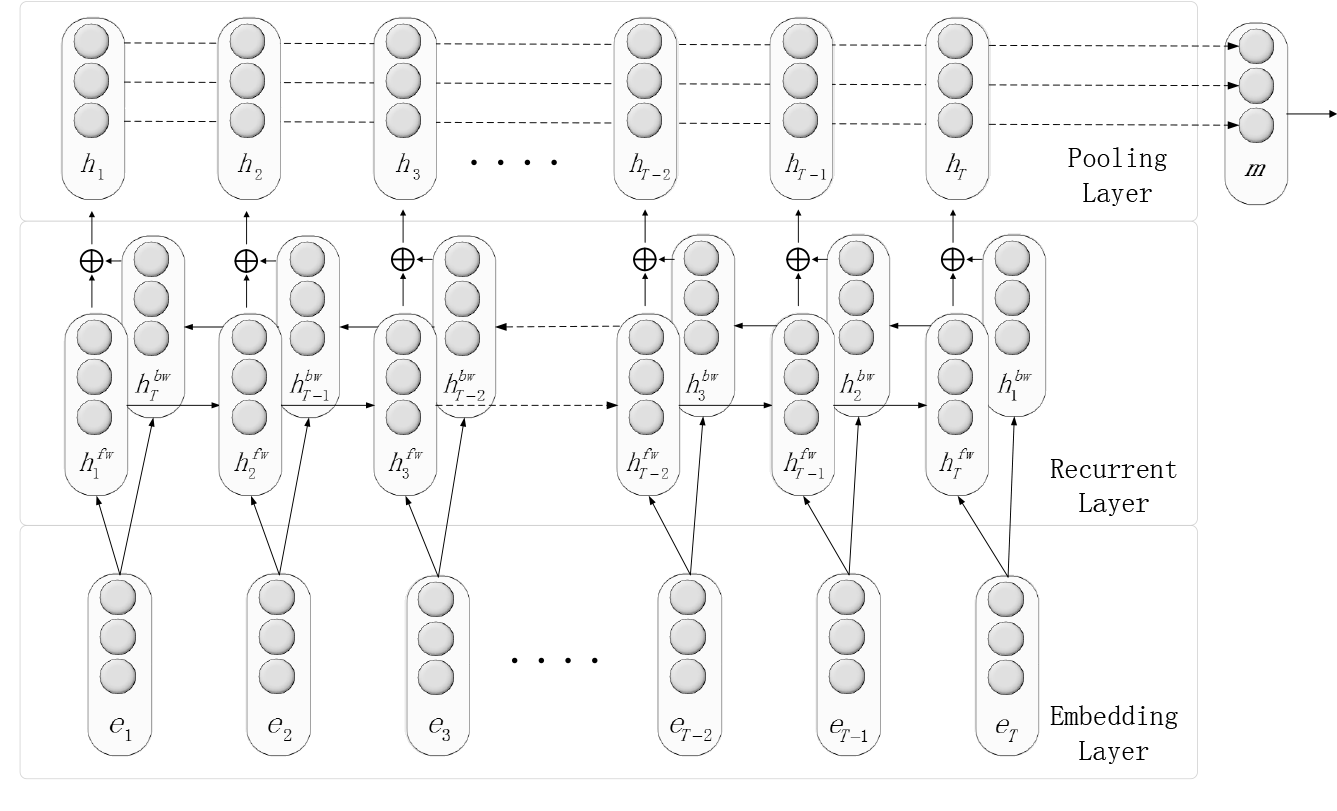
\includegraphics{blstm.png}
\end{figure}

The prediction result is given by the output layer with the activation function of softmax. Similar to aforementioned models, the loss function is the negative log-likelihood and the optimization is done by the stochastic gradient descent algorithm. In order to help propagating the gradient back to early steps easier, the fan-in technique is used to initialized the weights~\cite{plaut1987learning}. 

Compared with ConvNets-based approach which is the lack of capability to learning temporal features, the BLSTM shows a significant advantage in dealing with long-distance patterns. In addition, the semantic distribution of the BLSTM based model tends to be smoother than the one produced by the ConvNet-based model. 



\subsection{Attention Based Bidirectional Long Short-Term Memory Network}
However, BLSTMs are effective models in dealing with sequence, it still has some disadvantages. As not every word in the sequence has the same importance, BLSTMs do not have such ability to capture the most important semantic information in a sentence. The ideal classification model is expected to be able to automatically focus on the words that have decisive effective on the prediction results. Attention mechanism was proposed to tackle this problem. Combining BLSTM and attention mechanism, a attention-based BILSTM (Att-BLSTM) for classification was proposed and outperforms most of the existing approaches~\cite{zhou2016attention}. The structure of A-BLSTM is shown in Figure \ref{attention_blstm}. In this model, the forward and backward is combined by the element-wise sum. 

Firstly, we suppose $\mathbf{H}$ is the matrix which consists the output vectors $[\mathbf{h}_1, \mathbf{h}_2,...,\mathbf{h}_T]$from BLSTM, where $T$ is the length of the sentence. The representation $\mathbf{r}$ of the sentence is defined as 
\begin{equation}
\mathbf{M} = \mbox{tanh}(\mathbf{H})
\end{equation}
\begin{equation}
\mathbf{\alpha} = \mbox{softmax}(\mathbf{w}^{\intercal}\mathbf{M})
\end{equation}
\begin{equation}
\mathbf{r} = \mathbf{H} \mathbf{\alpha} ^\intercal
\end{equation}
where $\mathbf{H} \in \mathbb{R}^{d\times T}$, $d$ is the dimension of the word vector. The sentence-pair representation used for linear classification is in form of
\begin{equation}
\mathbf{y}^* = \mbox{tanh}(\mathbf{r})
\end{equation}

\begin{figure}
\caption{Model structure of attention-based bidirectional LSTM}
\label{attention_blstm}
\centering
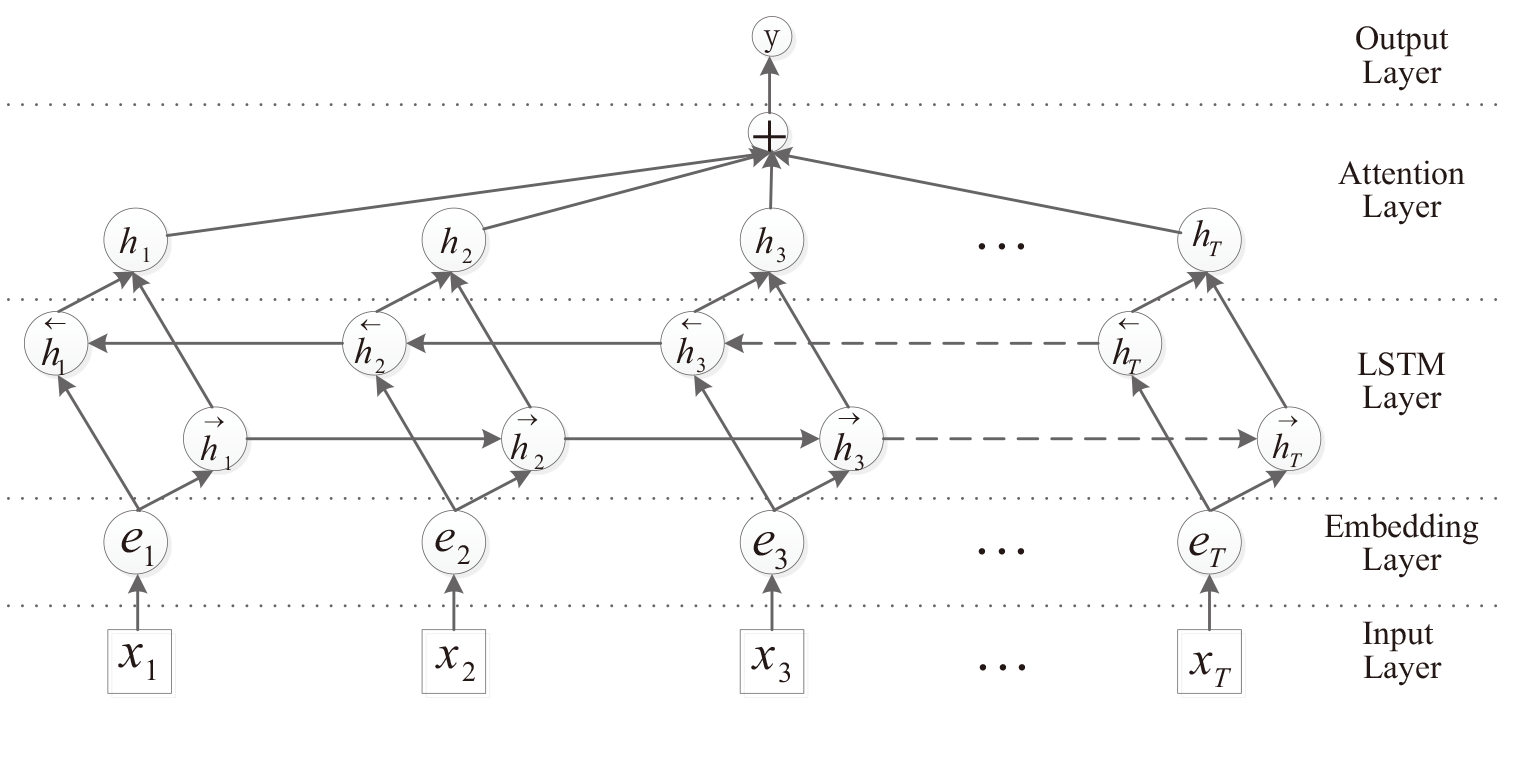
\includegraphics{attention_blstm.png}
\end{figure}

To avoid overfitting, A-BLSTM uses the nagative log-likelihood with L2 regularization:
\begin{equation}
L(\theta) = - \frac{1}{m} \sum_{i=1}^{m} t_i \mbox{log}(y_i) + \lambda \| \theta \|^2_F
\end{equation}
where $\mathbf{t}\in \mathbb{R}^m$ is the true label encoded as one-hot vector, $\mathbf{y}\in \mathbb{R}^m$ is the probability for each class produced by softmax function, $m$ is the number of classes, and $\lambda$ is the regularization hypeparameter which controls the penalty to the complex model.

In Att-BLSTM, dropout method is also used to do the regularization. During the training process, the dropout method is used on embedding layer and BLSTM layer. Dropout technique was first introduced by Hinton et al. in image classification\cite{krizhevsky2012imagenet}. It set the output of each neuron to zero with a specific probability. In this way, a part of neurons are dropped out and do not contribute to the forward and backward propagation. In Att-BLSTM, the dropout rate of embedding layer and LSTM layer is set as 0.3, 0.5 respectively.

The embedding layer is initialized by the pre-trained word embedding by Turian et al~\cite{turian2010word}. Other weights are initialized randomly. Different with aforementioned models which trained using stochastic gradient descent, Att-BLSTM is trained using AdaDelta~\cite{zeiler2012adadelta} with a learning rate of 1.0 and batch size of 10. The L2 regularization is set as $10^{-5}$.

Att-BLSTM achieve a similar result to the BLSTM which used many features derived from NLP tools and lexical resources~\cite{Zhang2015}. 



